\chapter{Études des paramètres}

\section{Approche du problème}

L'implémentation basée sur les graphes de calcul nous a permis de réaliser des tests sur les deux exemples introduits précédemment : XOR et MNIST. \`A travers de nombreux tests, nous avons souhaité étudier l'influence des paramètres de l'algorithme sur ses performances, c'est-à-dire sur sa précision et sa rapidité.
\medbreak
Il existe sept paramètres que l'on peut définir pour un réseau de neurones :
\begin{itemize}
\item l'architecture du réseau
\item le prétraitement des données
\item l'initialisation des poids
\item le choix des fonctions d'activation
\item le choix de la fonction de coût
\item la taille des batchs et le nombre de passage
\item le taux d'apprentissage
\end{itemize}
\medbreak
L'influence d'un paramètre n'étant bien évidemment pas indépendante ni des autres paramètres ni du problème considéré, il devient rapidement délicat d'obtenir des résultats généraux. En effet, il est impossible de réaliser des mesures en faisant varier sept variables en même temps, tout en effectuant des répétitions à chaque fois pour s'assurer de la précision des relevés. Pour s'affranchir de cette difficulté, nous avons choisi de ne faire varier qu'un seul paramètre à la fois en l'intégrant dans une configuration apportant des résultats acceptables. L'influence du paramètre étudié sur plusieurs configurations permet alors d'interpoler une estimation de son comportement général.
C'est donc ainsi que nous avons pu déterminer des éléments permettant de comprendre les rôles de ces paramètres et de les choisir pour optimiser l'efficacité d'un réseau de neurones. Ce sont ces éléments qui vont être présentés dans la suite de cette partie.

\section{\'Etude du XOR}

Dans un premier temps, nous avons effectués plusieurs tests sur un exemple très simple : XOR.
Quelques résultats ont déjà été présentés en partie \ref{resultat_premiere_implementation}. Ils vont être rappelés et détaillés ici.\\

Nous avons principalement étudié l'influence de l'architecture du réseau sur la rapidité de l'apprentissage. \\

La figure \ref{xor_architecture_tanh} présente la précision obtenue pour des structures d'une seule couche cachée avec un nombre variable de neurones de fonction d'activation tanh. Moins le réseau possède de neurones sur sa couche cachée, plus il a besoin d'apprendre sur un nombre important d'itérations. Cependant, avec seulement deux neurones sur la couche cachée, l'apprentissage se fait déjà relativement rapidement et le gain obtenu en ajoutant des états cachés n'est pas vraiment significatif puisqu'il ajoute un coût temporel de calcul.\\

Cette même étude réalisée dans les mêmes conditions en remplaçant simplement la fonction d'activation tangente hyperbolique par une ReLu donne des résultats complètement différents visible en figure \ref{xor_architecture_relu}. Ici, la taille de la couche cachée prend beaucoup plus d'importance puisqu'elle devient le paramètre principal pour obtenir une précision parfaite rapidement. En effet, même si augmenter le nombre d'itérations permet à des architectures avec peu d'états cachés permet d'améliorer la précision du réseau, cette amélioration est très lente. \`A l'inverse le réseau apprend presque instantanément lorsque l'on augmente le nombre d'états cachés.\\

\begin{figure}[!h]
\begin{center}
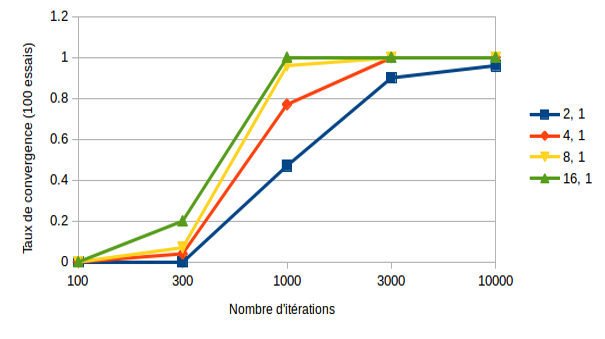
\includegraphics[scale=0.6]{images/chapter4/xor_architecture_tanh.png}
\caption{Convergence en fonction de l'architecture avec tanh}
\label{xor_architecture_tanh}
\end{center}
\end{figure}

\begin{figure}[!h]
\begin{center}
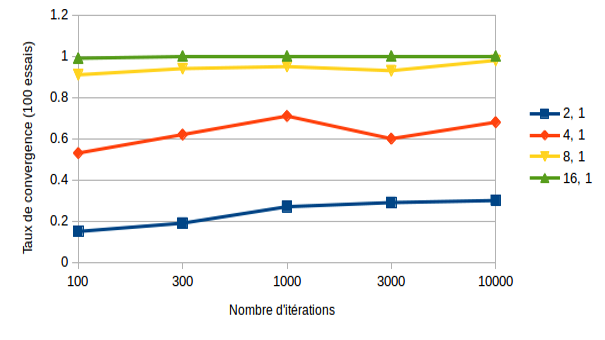
\includegraphics[scale=0.6]{images/chapter4/xor_architecture_relu.png}
\caption{Convergence en fonction de l'architecture avec relu}
\label{xor_architecture_relu}
\end{center}
\end{figure}

L'exemple de ces deux situations représente clairement les problèmes rencontrés pour étudier les influences des paramètres d'un réseau de neurone. En effet, l'influence de la taille de la couche cachée sur notre réseau n'est plus du tout la même selon le choix de la fonction d'activation appliquée à chaque neurone. Ainsi, il n'est souvent pas possible de définir une règle générale à appliquer concernant un paramètre pris indépendamment des autres.

\section{\'Etude de MNIST}

\subsection{Introduction}
Dans cette partie, mis à part les paramètres explicitement précisés pour un exemple, toutes les mesures qui vont être présentées furent réalisées en utilisant les paramètres suivants :
\begin{itemize}
\item Pas de couche cachée, les neurones d'entrée sont directement reliés aux sorties
\item Les entrées sont centrées et normalisées : chaque pixel est alors représenté par une valeur de [-1;1]
\item Les poids sont initialisés aléatoirement avec une fonction Gaussienne centrée de variance 0,1
\item On utilise une sigmoïde en sortie
\item On utilise l'erreur quadratique pour la fonction de coût
\item Les exemples sont traités pas batch de 128
\item On fixe un learning rate de 0,1
\end{itemize}

\subsection{Architecture du réseau}

Le nombre de couches cachées d'un réseau de neurones ainsi que leur composition constitue l'architecture de ce réseau.

De façon intuitive, il parait évident qu'une plus grande architecture de réseau, possédant plus de neurones par couches cachées ou plus de couches cachées apprendra avec plus de précision l'ensemble de données. Cependant cela a un coût en temps et rendra l'apprentissage beaucoup plus lent.
Ainsi, alors qu'un apprentissage effectué sans couche cachée sur 30 passages du set de données mnist aura une précision d'environ 93\%, un réseau composé d'une couche cachée de 400 neurones ayant pour fonction d'activation tangente hyperbolique pourra avoir sur ce même ensemble presque 98\% de précision. Le résultat de cette seconde situation est visible en figure \ref{mnist100}. On y remarque que l'ensemble de données est très rapidement complètement appris.
\begin{figure}[!h]
\begin{center}
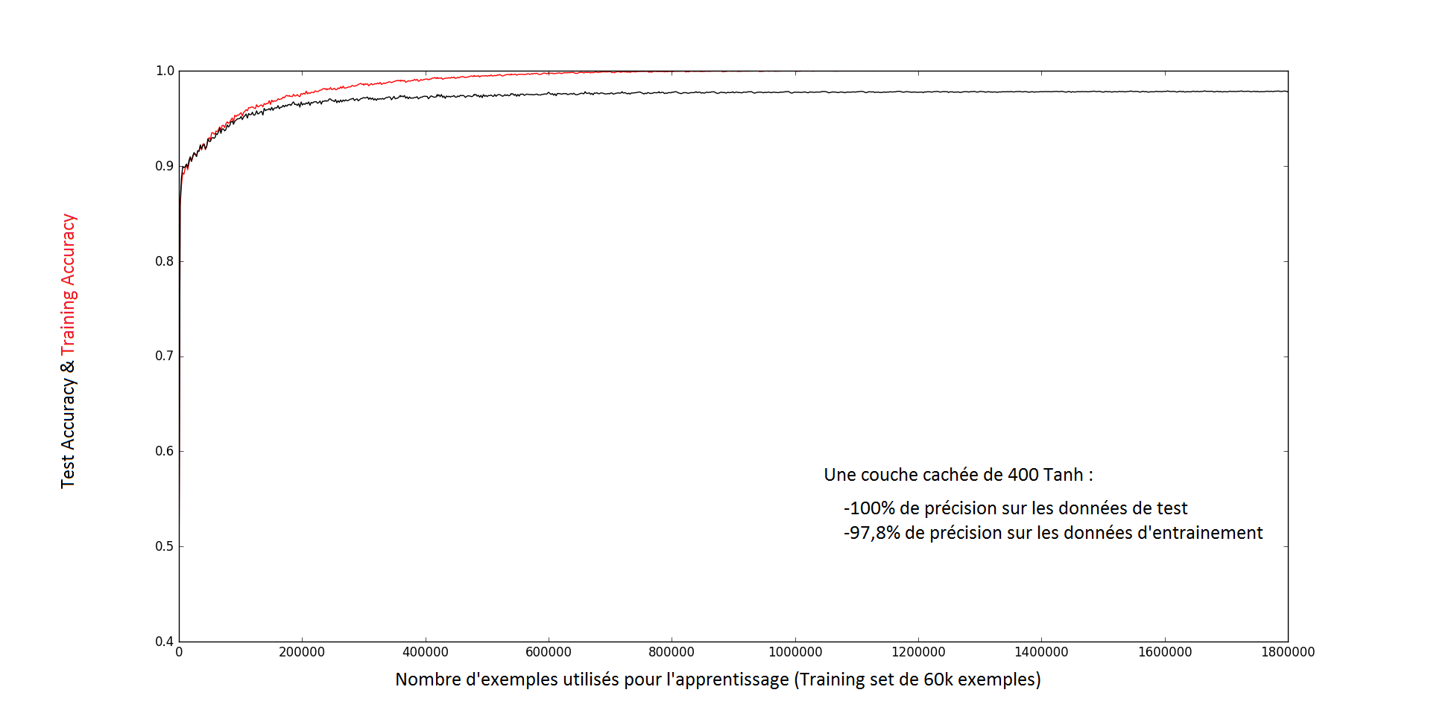
\includegraphics[scale=0.5]{images/chapter4/mnist100.png}
\caption{Précision pour un réseau avec une couche cachée de 400 neurones}
\label{mnist100}
\end{center}
\end{figure}

\subsection{Initialisation des poids}
Avant le lancement de l'algorithme sur un réseau de neurone, il est nécessaire d'initialiser les poids. L'usage le plus courant est de les initialiser aléatoirement. Cependant, le choix de la distribution aléatoire n'est pas forcément évident. En effet, on peut choisir d'utiliser une distribution uniforme, une distribution gaussienne ou tout autre type de distribution aléatoire avec des paramètres variables.

Nous avons donc testé trois types de fonction d'initialisation des poids : une répartition uniforme, une répartition uniforme centrée en 0  et une répartition gaussienne centrée en 0.
Si les initialisations centrées en 0 permettent une convergence un petit peu plus rapide, ces trois initialisations produisent des résultats similaires. Cependant, l'amplitude des poids change beaucoup les résultats quelle que soit la fonction d'initialisation. En effet, les poids convergeant lors de l'apprentissage vers de petites valeurs, une initialisation avec de petites amplitudes va permettre une convergence plus rapide.

\begin{figure}[!h]
\begin{center}
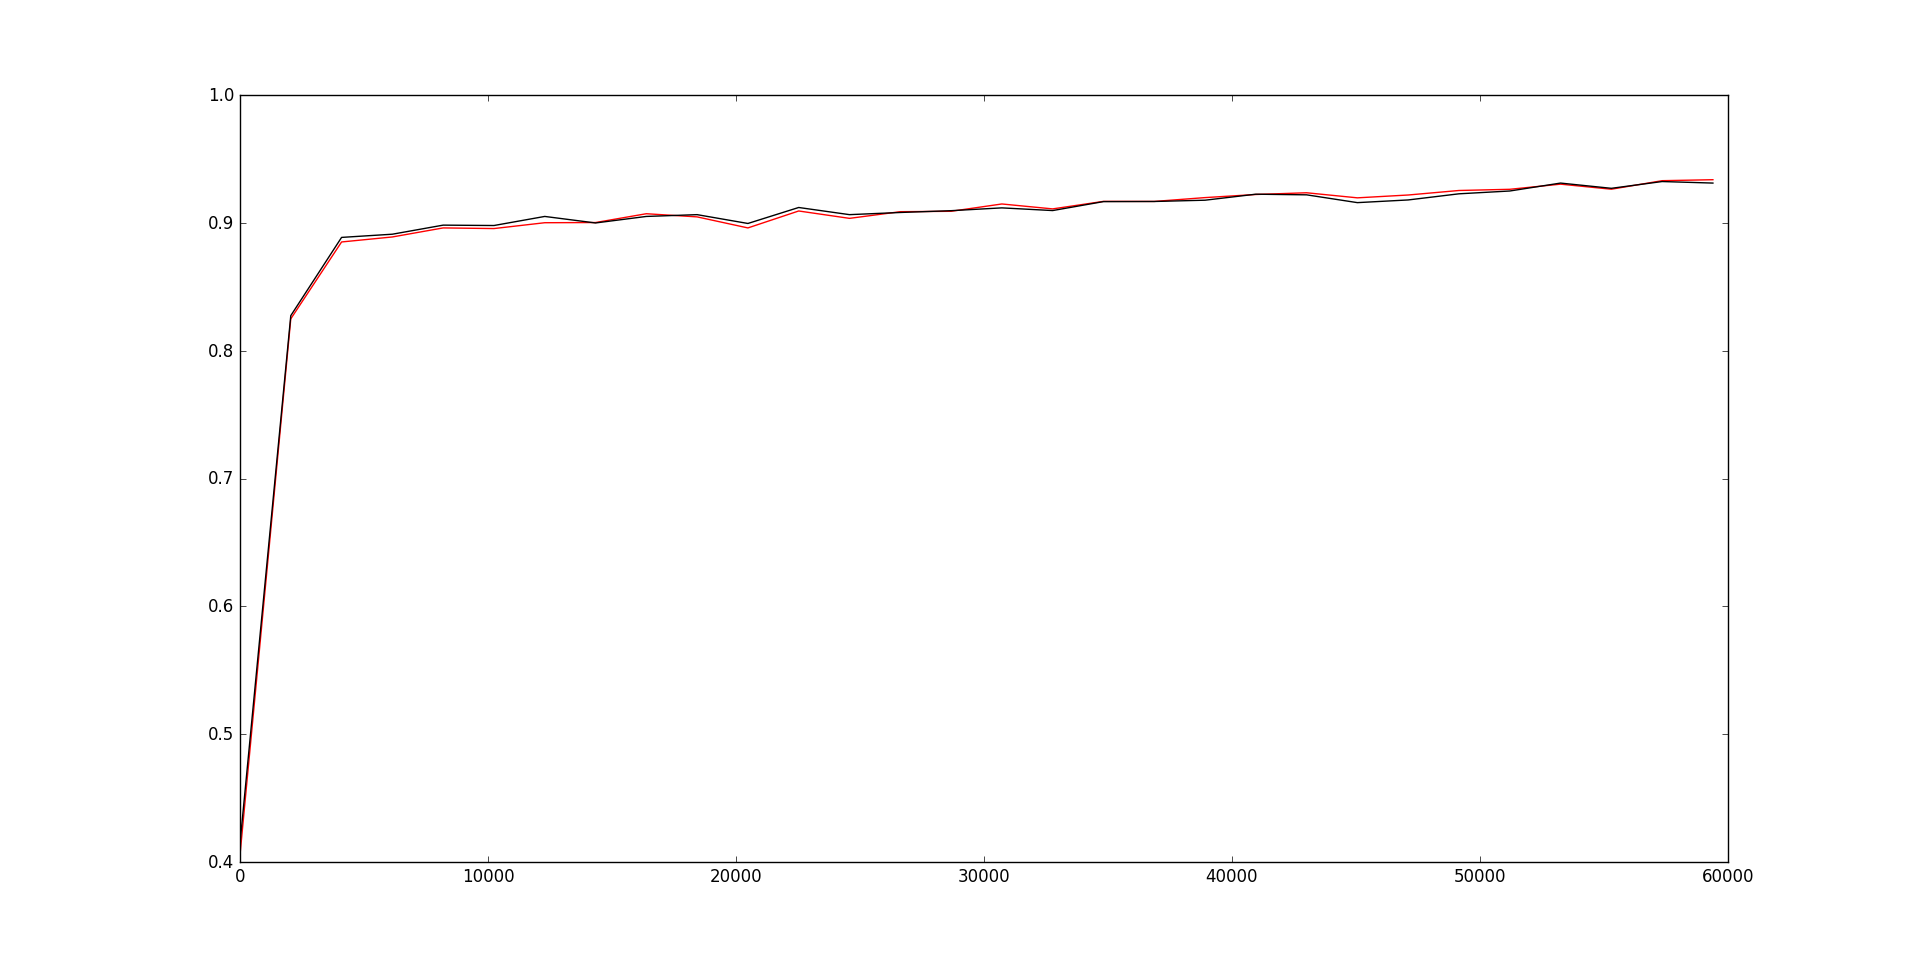
\includegraphics[scale=0.2]{images/chapter4/initialisationpoids_amplitude01.png}
\caption{Précision sur les ensembles de test (en noir) et d'apprentissage (en rouge) en fonction du nombre d'exemples utilisés pour l'apprentissage pour une initialisation des poids d'amplitude 0.1 }
\label{initialisationpoids_amplitude0.1}
\end{center}
\end{figure}

\begin{figure}[!h]
\begin{center}
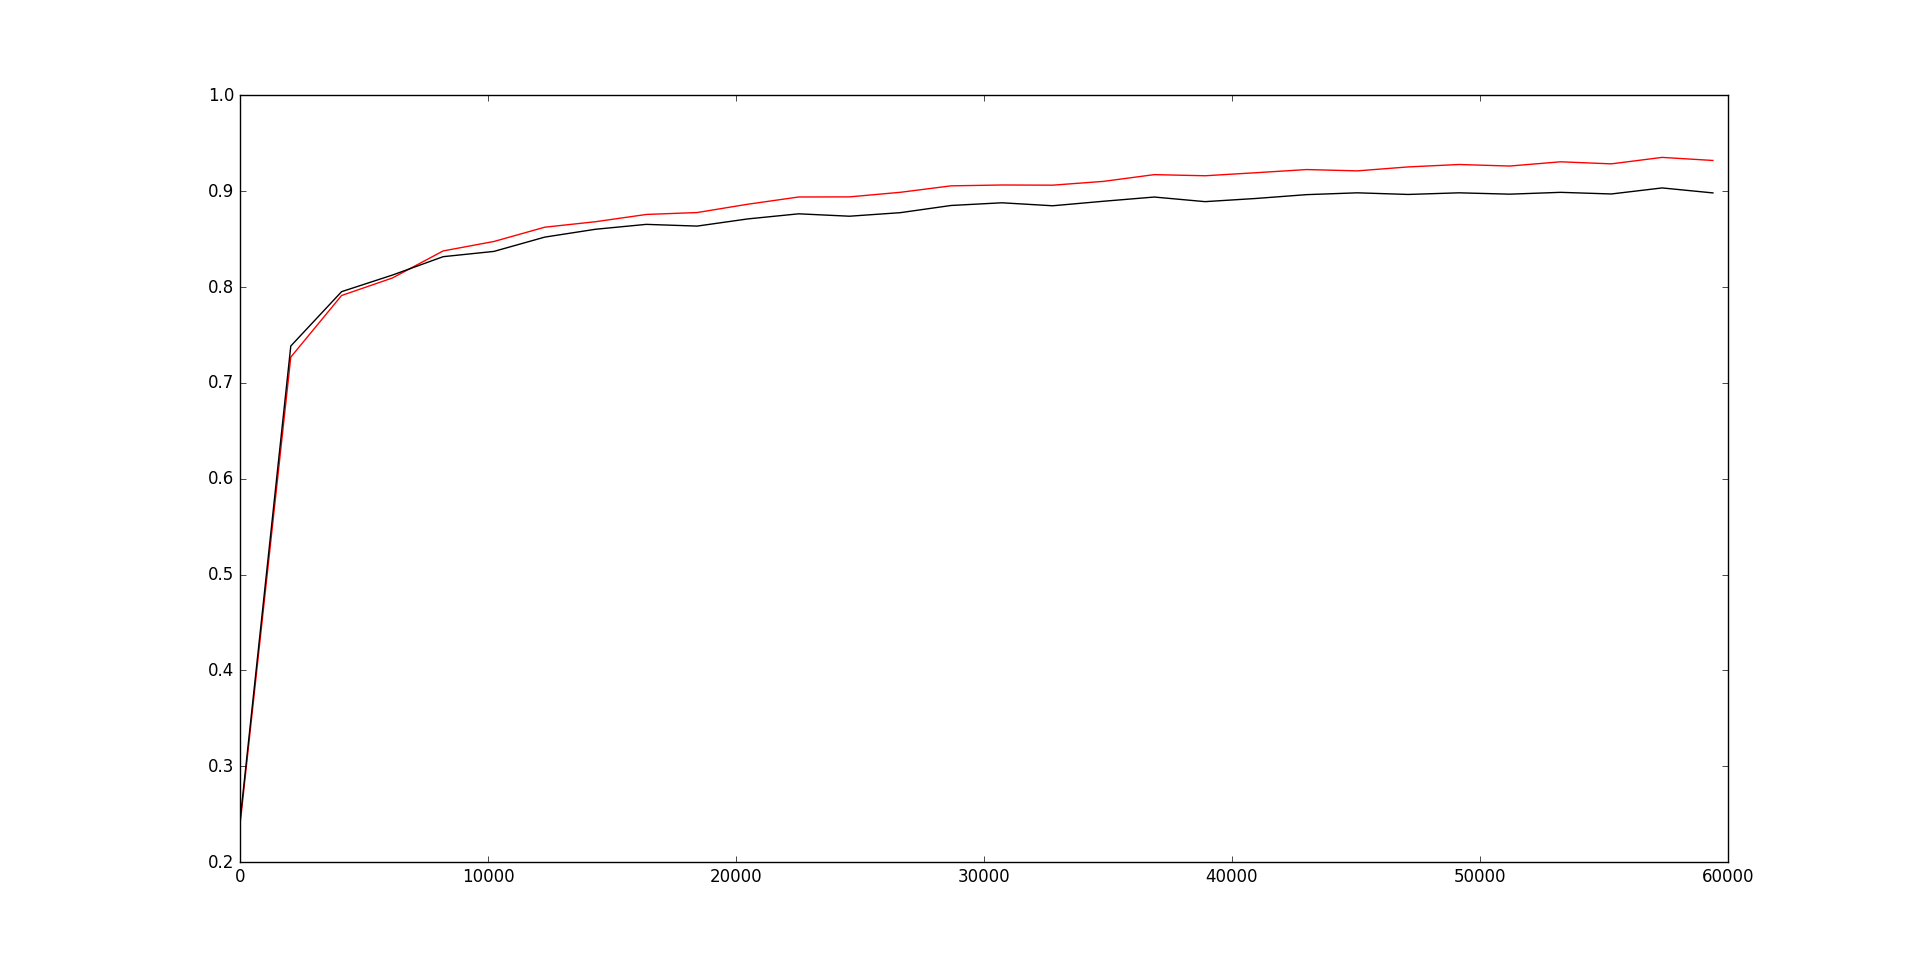
\includegraphics[scale=0.2]{images/chapter4/initialisationpoids_amplitude10.png}
\caption{Précision sur les ensembles de test (en noir) et d'apprentissage (en rouge) en fonction du nombre d'exemples utilisés pour l'apprentissage pour une initialisation des poids d'amplitude 10}
\label{initialisationpoids_amplitude10}
\end{center}
\end{figure}

C'est ce que l'on peut voir sur les deux figures \ref{initialisationpoids_amplitude0.1} et \ref{initialisationpoids_amplitude10}. Dans les deux cas, les poids sont initialisés selon une loi normale centrée de variance 0,1. Cependant, sur la première, un coefficient multiplicatif de 0,1 leur est affecté alors que celui-ci est de 10 sur la deuxième.
On peut ainsi bien observer que dans le cas du facteur multiplicatif de 10, la convergence est plus lente au début de l'apprentissage, même si l'on atteint sensiblement les mêmes valeurs finales de précision.



\subsection{Choix des fonctions d'activations et de coût} 
 
Le tableau \ref{influence_fonction_cout} présente quelques résultats sur la précision obtenu par le réseau selon les fonctions de coût et les fonctions en sortie utilisées.\\ 
\begin{center} 
\begin{tabular}{|c|c|c|c|c|} 
\hline 
Sortie & \multicolumn{2}{| c |}{Softmax} & \multicolumn{2}{|c|}{Sigmoïde}\\ 
\hline 
Fonction & Entropie & Erreur & Entropie & Erreur \\ 
de coût & croisée & quadratique & croisée & quadratique\\ 
\hline 
Moyenne & 0,92303 & 0,92667 & 0,9149 & 0,91708\\ 
\hline 
Écart-type & 0,00033350 & 0,00056578 & 0,00025820 & 0,00028597\\ 
\hline 
Intervalle 95\% & 0,00020670 & 0,00035067 & 0,00016003 & 0,000177242\\ 
\hline 
\end{tabular} 
\captionof{table}{Influence de la fonction de coût} 
\label{influence_fonction_cout} 
\end{center} 
 
Le choix de la fonction de coût ne semble avoir qu'un impact très mineur sur les résultats obtenus par le réseau. L'erreur quadratique présente des performances légèrement supérieures à l'entropie croisée pour ce problème mais cette différence est très faible. 
 
En revanche il apparait que l'utilisation de la fonction Softmax en sortie donne de meilleurs résultats que celle d'une sigmoïde. L'emploi de Softmax entrainant un cout en temps plus important que celui de Sigmoïde, cet avantage est à relativiser. 
 
\subsection{Taille des batchs et nombre de passages} 
 
La taille d'un batch est le nombre d'exemples que l'on insère dans le réseau entre chaque rétropropagation du gradient.\\ 
 
 
\begin{figure}[!h] 
\begin{center} 
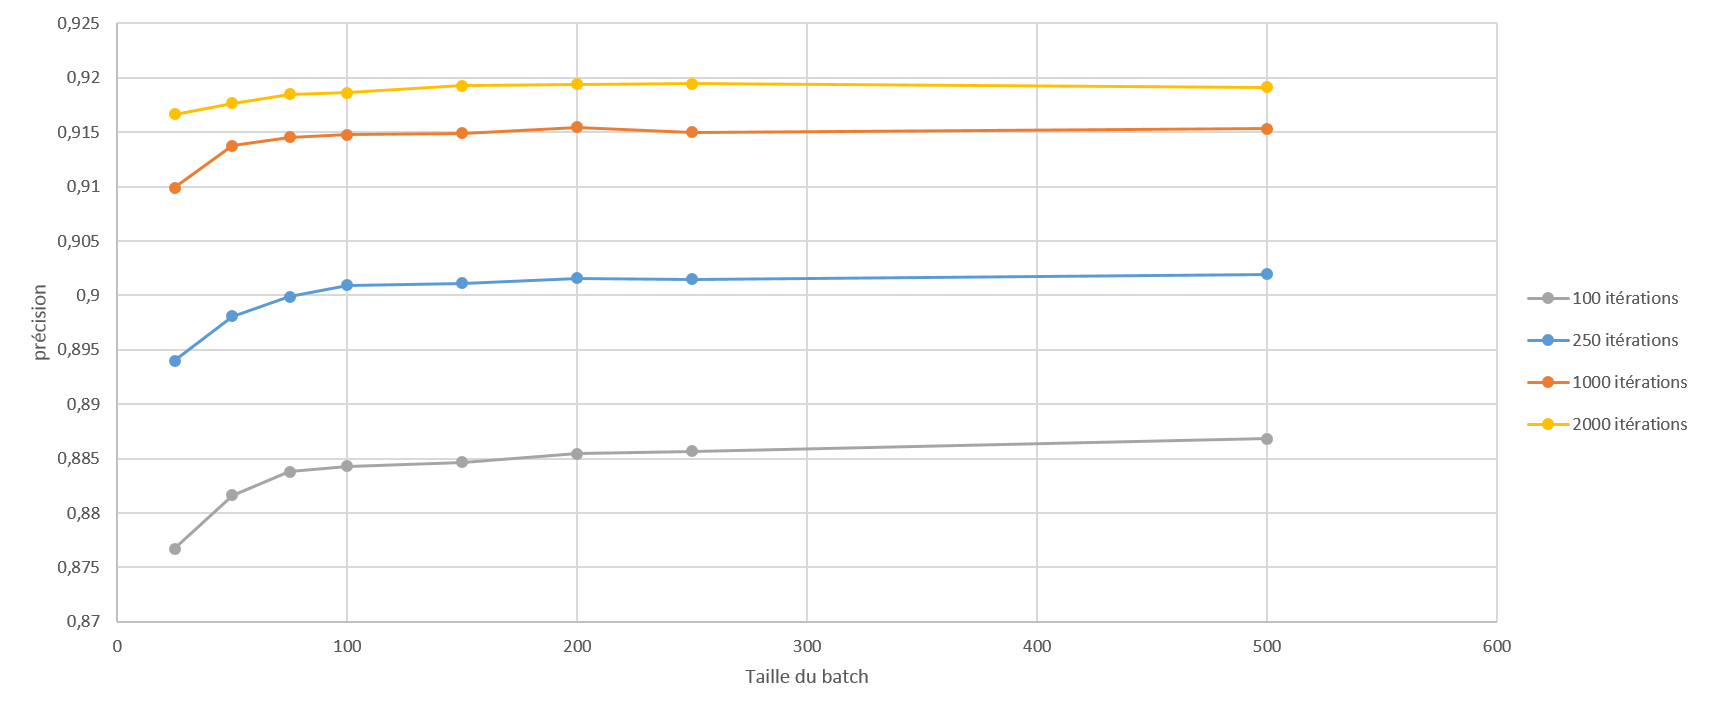
\includegraphics[scale=0.5]{images/chapter4/precision_taille_batch.png} 
\caption{Influence de la taille du batch} 
\label{precision_taille_batch} 
\end{center} 
\end{figure} 
 
\begin{figure}[!h] 
\begin{center} 
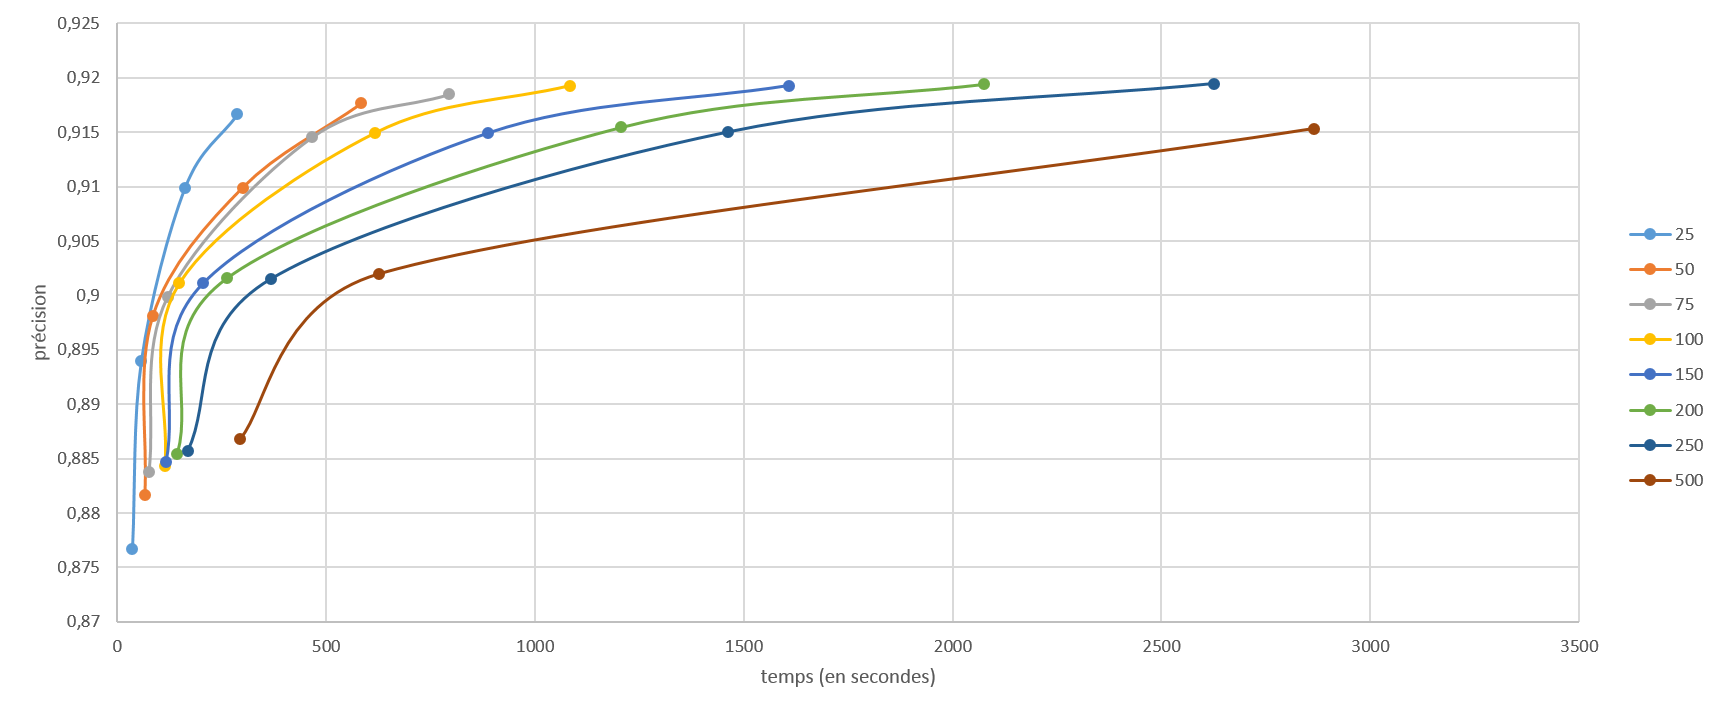
\includegraphics[scale=0.5]{images/chapter4/precision_batch_temps.png} 
\caption{Influence de la taille du batch sur le temps de calcul} 
\label{precision_batch_temps} 
\end{center} 
\end{figure} 
 
La figure \ref{precision_taille_batch} présente la précision obtenue pour différentes tailles de batch. La figure \ref{precision_batch_temps} présente ces mêmes données mais réparties en fonction du temps de calcul.\\ 

On retrouve les principales influences de l'utilisation d'une descente de gradient par batch plutôt que stochastique. En effet, plus le batch est de taille faible, plus le réseau va apprendre rapidement et converger vers sa précision finale dans un temps de calcul réduit. En revanche, utiliser des batchs permet d'améliorer la précision finale et la stabilité des résultats. \\
 
La dernière figure \ref{efficacite_batch} présente, pour l'apprentissage des $60000$ données de l'ensemble d'apprentissage de mnist, les précisions moyennées sur 20 tests en fonction de la taille du batch utilisé. On retrouve bien le plus grands écart-types pour des petits batchs. La taille de batch optimale pour le problème mnist avec notre configuration peut donc être estimée à 50. 
 
\begin{figure}[!h] 
\begin{center} 
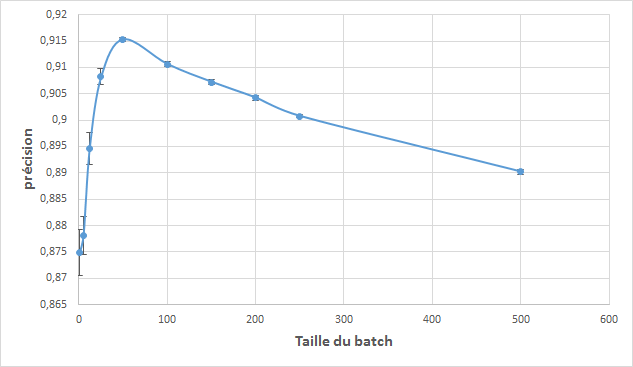
\includegraphics[scale=0.7]{images/chapter4/efficacite_batch.png} 
\caption{Influence de la taille du batch sur la précision} 
\label{efficacite_batch} 
\end{center} 
\end{figure} 

\subsection{Taux d'apprentissage}
Nous avons aussi étudié l'influence du taux d'apprentissage ou learning rate. En effet celui-ci influe sur la mise à jour des poids : plus il est grand et plus chaque l'importance donnée au calcul de la dérivée est important. Avoir un taux d'apprentissage grand permet d’obtenir rapidement des performances satisfaisantes en termes de précision. Au contraire, des phénomènes d'oscillations sont observés pour un apprentissage conséquent, et cela fournit en retour de moins bons résultats, par rapport à des taux d'apprentissage plus faibles. Cela a été illustré sur la figure \ref{influence_learningrate}.

\begin{figure}[!h]
\begin{center}
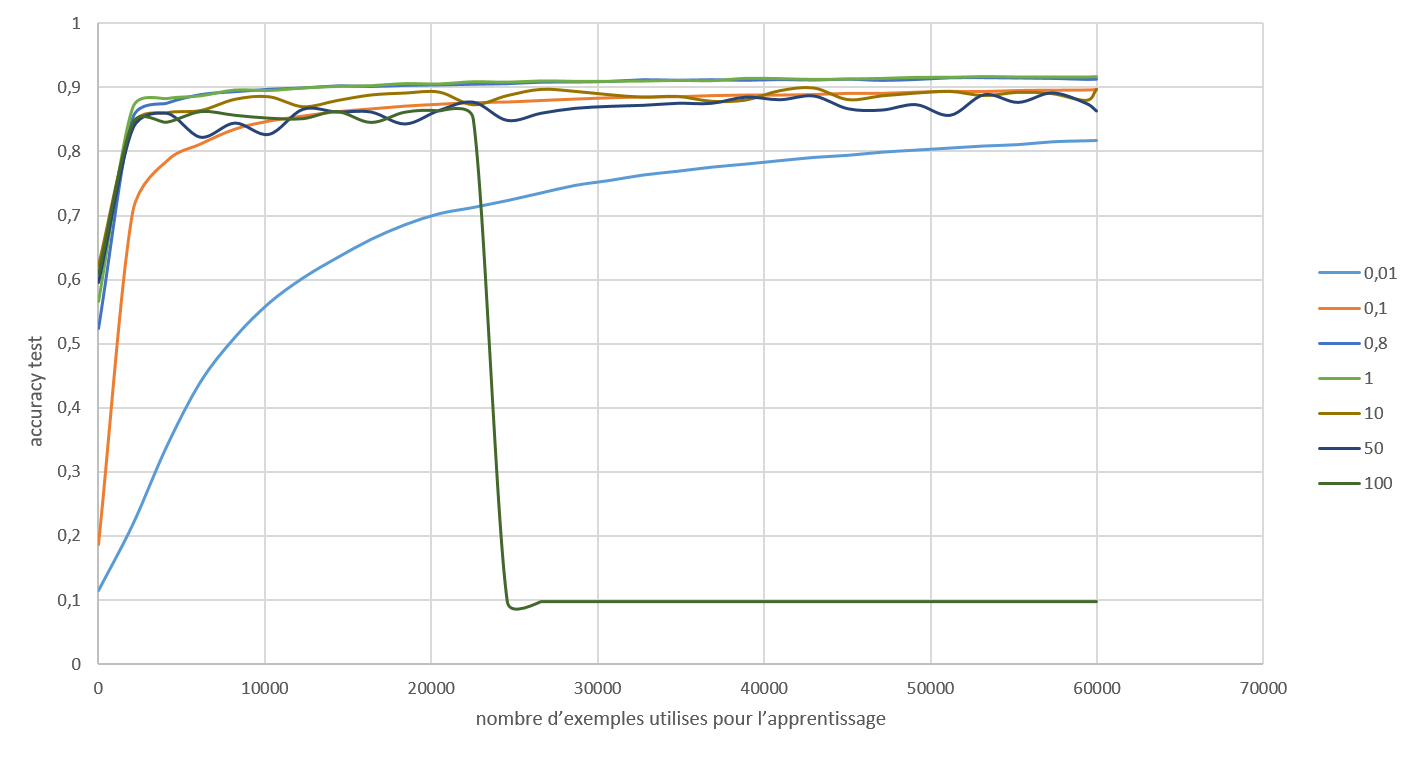
\includegraphics[scale=0.6]{images/chapter4/influence_learningrate.png}
\caption{Influence du learning rate sur la précision sur l'ensemble de test en fonction du nombre d'exemple utilisés}
\label{influence_learningrate}
\end{center}
\end{figure}

Nous avons alors étudié l'apprentissage du réseau pour des taux d'apprentissage allant de 0.01 à 100.
Nous pouvons alors distinguer trois cas reflétant les principaux comportements :

\begin{itemize}
\item Pour un taux d'apprentissage de 0.01, la convergence est très lente mais sans oscillations. Si la précision obtenue peut-être à hauteur des autres taux d'apprentissage en utilisant plus d'exemples, on peut considérer celui-ci trop petit.
\item Pour un taux d'apprentissage de 100, la convergence est très rapide au début, mais oscille beaucoup et va finalement bloquer l'apprentissage vers un autre minimum local de coût non désiré. On peut donc considérer ce taux d'apprentissage comme trop grand.
\item Pour un taux d'apprentissage de 0.1, il semble apparaître un bon compromis entre stabilité et vitesse de la convergence. C'est cette valeur qui en général sera choisie pour les tests, bien que d'autres soient satisfaisants (0.8 ou 1 par exemple).
\end{itemize}